\documentclass[12pt]{article}
\usepackage{amsmath}
\usepackage{graphicx}
\usepackage{caption}
\usepackage{subcaption}

\begin{document}
\section{Data Analysis}
\subsection{Introduction}
The previous chapter explained the setup of the experiment. We now discuss the analysis of the data, where we looked for peaks in the recorded spectra.  In the absence of statistically significant peaks, we set a limit on the minimum detectable power we can measure, and use that as our exclusion limit. 

%In our analysis, we assume that the axion has a boosted Maxwellian distribution with energy fractional width of $\mathcal{O}(10^{-6}$, or about one 34 KHz bin. 

The analysis process can be decomposed into three parts: baseline corrections, weighting and peak finding.

In section 4.2 we show the procedure for correcting the raw data and cuts made. Section 4.3 discusses the power combining and resulting exclusion limit, section 4.4 describes the resulting candidates and section 5 shows our final exclusion result.

\section{Data Processing}


In a typical run, we sampled voltage as a function of time from two channels in our receiver chain over the course of an hour. At a sampling rate of 10 MHz/sec, this generated a large volume (37 GB  per channel) of data. Using the FFTW libraries \cite{fftw} we computed the discrete Fourier transform for each set of 294 samples. Squaring the voltage transforms and summing resulted in a power spectra. The double-sided power spectra has a span of -5 to 5 MHz, centered at 0 MHz. Each spectra is saved to a file which consists of two vectors corresponding to the baseband frequency and power density, respectively. The first step in data analysis is to extract axion induced signals (i.e. peaks) from raw spectra. As we are searching for extremely weak signals amidst the noise, searching for true signals is a challenging task. 

An axion induced signal would appear as a local maxima in the spectra. However, detecting the signal is challenging as a the weakness of the signal means it may be buried by noise, causing a high false positive rate of peak detection. For each cavity setting, we average over many spectra to increase our sensitivity. As well, electronic noise results in a curve that affects the background of the data, which is referred to as a baseline. THe existence of the baseline produces strong  bias in the peak detection. It is desirable to remove the baseline before peak detection.

\begin{figure}[htbp]
\includegraphics[width=\linewidth]{flowchart2}
\caption{Data Analysis Pipeline}
\end{figure}

\section{Baseline correction}

Baseline correction is typically a two-step process: (1) estimating the baseline and (2) subtracting the baseline from the signal. In the following, we list details of the method we used to calculate the baselines using smoothing filters.

\subsection{Smoothing Filters}

For an input spectrum, we represent it as [f,p] with the first element as the frequency bin vector and the second element as the power spectral density (with equal length). We use p[n] to denote the discrete form of the power density vector. The input spectrum is always discrete. A spectrum after smoothing can be expressed as $y[n] = x[n] * w[n]$ where $*$ denotes the convolution operation. In the above equations, $w[n]$ is a weight vector. The use of different $w[n]$ will lead to different filters.

\subsection{Moving average filter}

The baseline was initially estimated using a moving average filter, where the output of the moving average filter $y[n]$ is defined as:

\begin{align*}
y[n] = x[n] * w[n] = \frac{1}{2k+1}\Sigma_{i=-k}^{k} x[n-i]
\end{align*}

where $w[n] = \frac{1}{2k+1}$, $-k \leq n \leq k$ a. The odd number $2k+1$ denotes filter width. The greater the filter width, the more intense the smoothing effect. However, this filter failed to remove oscillatory structure that appears at the level of $O(10^{-3})$. Shown below is the residual after using the moving average to calculate the baseline and then averaging over 522 baseline-removed traces.

This structure is much wider than our expected signal; therefore, we attempt to correct for it using a different filter, known as a Savitzky-Golay filter. The Savitsky-Golay filter can be considered as a generalized moving average filter. It performs a least squares fit of a small set of consecutive data points to a polynomial and takes the central point of the fitted polynomial curve as output.

The smoothed data point $y[n]$ after the Savitzky-Golay filtering is given by the following equation:

\begin{align*}
y[n[ = x[n] * w[n] = \frac{\Sigma A_i x[n-i]}{\Sigma A[i]}
\end{align*}

Using the Savitzky-Golay filter with a polynomial order of 4 and window size of 11 points reduces the residual structure significantly.

\begin{figure}[htbp]
\centering
\begin{subfigure}{\textwidth}
\includegraphics[width=0.8\linewidth]{01-11-08-24-55avgsubpltposfreq_522}
\caption{Systematic residual structure seen when baseline is estimated using moving average filter.}
\end{subfigure}
\begin{subfigure}{\textwidth}
\includegraphics[width=0.8\linewidth]{01-11-08-24-55gs-avgsubpltposfreq_522}
\caption{Residual when baseline is estimated using Savitzky-Golay filter.}
\end{subfigure}
\end{figure}

\section{Data Description}

We use data from measurements taken between 12/13 and 6/14. The physical temperature of the cavity was between 4 and 10 K. The observation time for each cavity setting was on average 1.06 hours. For data taken between Jan 29 2014 and March 13 2014, a test tone signal was injected into the cavity. The test tone frequency was set to be mixed down to -1 MHz. For these runs the cavity frequency was normally mixed down to 2 MHz. 

This data set has 499 groups of data. Each group has a number of spectra, usually 261. 
%\section{Running Time}
%
%\section{Parameter Tuning}
%
%\section{Conclusion}
%
%\begin{table}
%\centering
%\begin{tabular}{| c | c | c | c |}\hline
%\hline
%Component & Gain (dB) & \multicolumn{1}{|p{2cm}|}{\centering Power Density \\ (dBm/Hz)} & Total Power (dBm) \\ \hline \hline
%Cavity & - & -185 & -  \\ \hline
%Cryogenic Amplifiers w/ 3dB atten. & 50 & -144 & - \\ \hline
%Waveguide to Shielded Room & -3.4 & -148.6 & -\\ \hline
%RF switch & -2.7 & & \\ \hline
%RF filter & -0.2 & - & -\\ \hline
%RF mixer & -12 & x & x\\ \hline
%Cable to Electronics & - & - & - \\ \hline
%16 dB attenuation & -16 & - & - \\ \hline
%1.5 GHz Bandpass Filter & -0.5 & - & - \\ \hline
%4 GHz Amplifier & 59.5 & - & - \\ \hline
%Bandpass Filter & -0.5 & - & - \\ \hline
%4 GHz - 590 MHz Mixer & -6.5 & - & - \\ \hline
%25 MHz Bandpass Filter & -2.3 & - & - \\ \hline
%590 MHz Amplifier  & 34 & - & - \\ \hline
%25 MHz Bandpass Filter & -2.3 & - & - \\ \hline
%590 Mz to DC IQ Mixer & -8.5 & x & x \\ \hline
%4 MHz Low Pass Filter & x & - & - \\ \hline
%50 Ohm Voltage Pre-Amp  & x & - & - \\ \hline
%\end{tabular}
%\caption{Power levels at different points (in dBm) in the receiver chain. At each point in the receiver chain the total broadband noise power over the bandwidth of the next component is insufficient to cause saturation}
%\label{table:rxchain}
%\end{table}

The measurements from Dec 2013 to May 2014 were taken at 368 distinct resonant frequencies, with 499 total observations made. 415 of these observations were taken for 1.06 hours, with a smaller number (28) being taken for longer observation times; the remaining observations were taken for shorter times due to storage limitations or technical problems with the data acquisition system, and later were retaken to increase the number of averages at that frequency setting. For each measurement we tracked the in-phase and quadrature components of the baseband signal, and converted the time-domain data into a 294 bin,  34013.6 Hz/bin double-sided FFT power spectra. The FFT traces are 10 MHz wide, with a center frequency at 0Hz. Each of the spectra consist of 500,000 averages lasting a total of 14.7 seconds in integration time; for the standard observation length of 1.06 hrs, 261 such spectra could be produced. 

\begin{figure}[htbp]
\centering
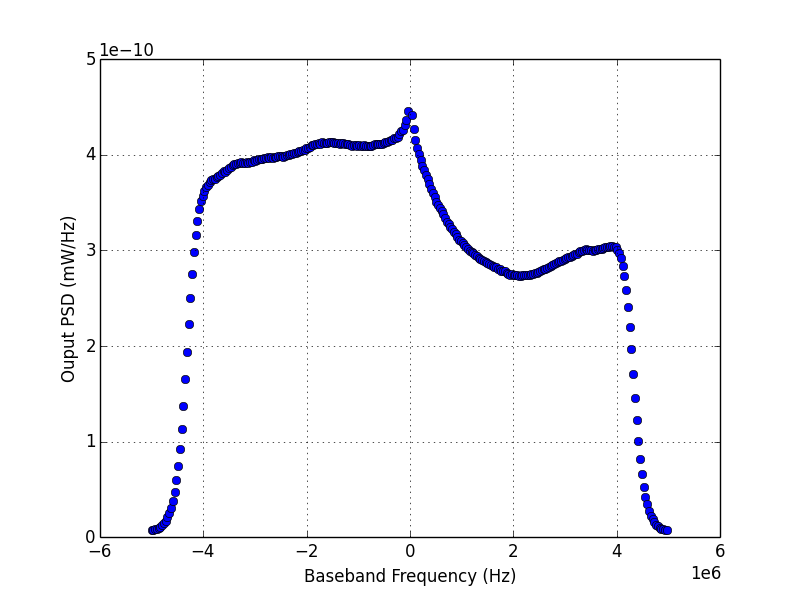
\includegraphics[width=\textwidth]{examplespectra}
\label{fig:example}
\caption{FFT Power spectral density vs baseband frequency. Each bin is 34013.6 Hz wide.}
\end{figure}

Shown in Figure\ref{fig:example} is one such raw FFT trace. The horizontal axis shows the baseband frequency, and the vertical axis corresponds to the power density across the 50 ohm input in milliWatts per Hz. The visible features in the spectrum are the spike at 0 Hz, which is DC noise, the skirts at the edges showing the attenuation of the last low pass filter in the receiver chain, the 1/f noise near the center, and a dip corresponding to the combined cavity-amplifier response.

\subsection{Corrections}

To remove the features due to the last low-pass filter, we cut out the first and last thirty bins of each trace to remove the filter skirts, and also cut out twenty bins around the center to remove the DC spike and 1/f noise. 

%\begin{figure}[htbp]
%\centering
%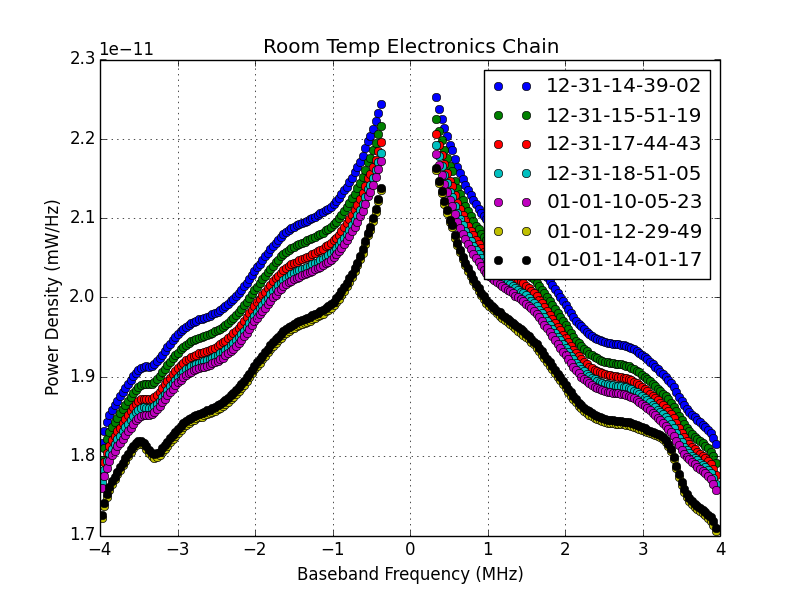
\includegraphics[width=\textwidth]{roomtempchain1}
%\label{fig:roomtempchain1}
%\caption{The transfer function of the room temperature electronics chain with the RF switch in place, for different settings of the first local oscillator.}
%\end{figure}

The first local oscillator of the receiver is usually set so that the cavity resonant frequency is mixed down to 2 MHz. However, for a period of runs the first local oscillator was set so that the cavity frequency was mixed down to -1 MHz or -0.5 MHz in the baseband. There are also some measurements that had to be discarded because the local oscillator frequency was incorrectly set due to operator error and thus the cavity frequency was outside of the pass-band of the last filter. In order to prevent this from occurring, we introduced a test tone signal at an RF frequency such that it would mix down to -1 MHz, to make sure the local oscillator was set correctly. For the measurements taken with the test tone on, we later also cut out the bin with the test tone signal, as well as the two nearest bins to either side, for reasons to do with the fit. Lastly, there is some leakage into the positive frequency bins at 1 MHz due to the test tone; this will be discussed later.

\begin{figure}[htbp]
\begin{subfigure}{0.5\linewidth}
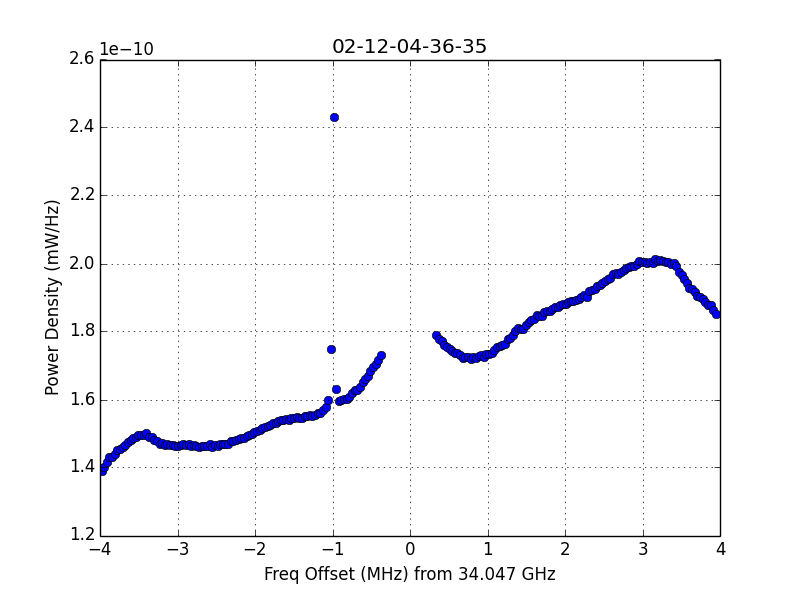
\includegraphics[width=\textwidth]{rawwithtesttone}
\caption{FFT trace with test tone signal at 34.044 GHz, -60 dBm}
\end{subfigure}
\begin{subfigure}{0.5\textwidth}
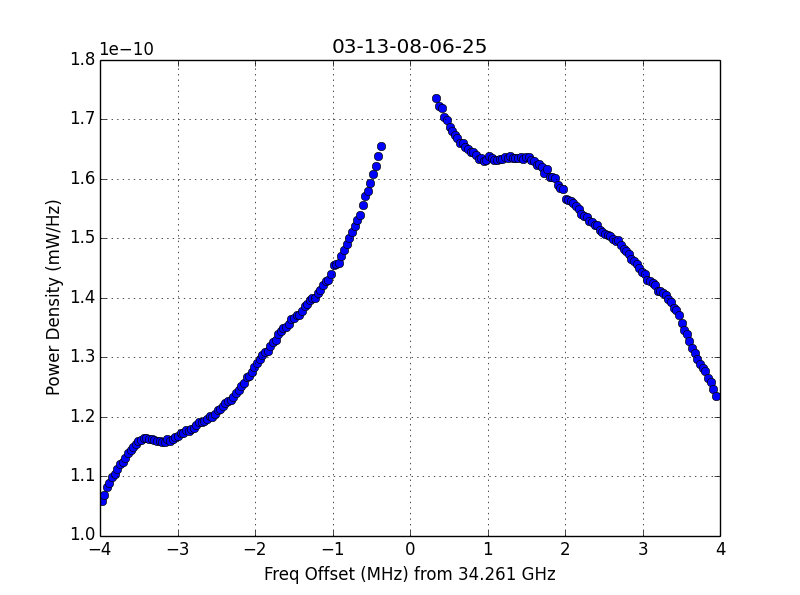
\includegraphics[width=\textwidth]{rawwithtesttone2}
\caption{FFT trace with test tone signal at 34.258 GHz, -72 dBm}
\end{subfigure}
\label{fig:testtone}
\end{figure}

\begin{figure}[htbp]
\centering
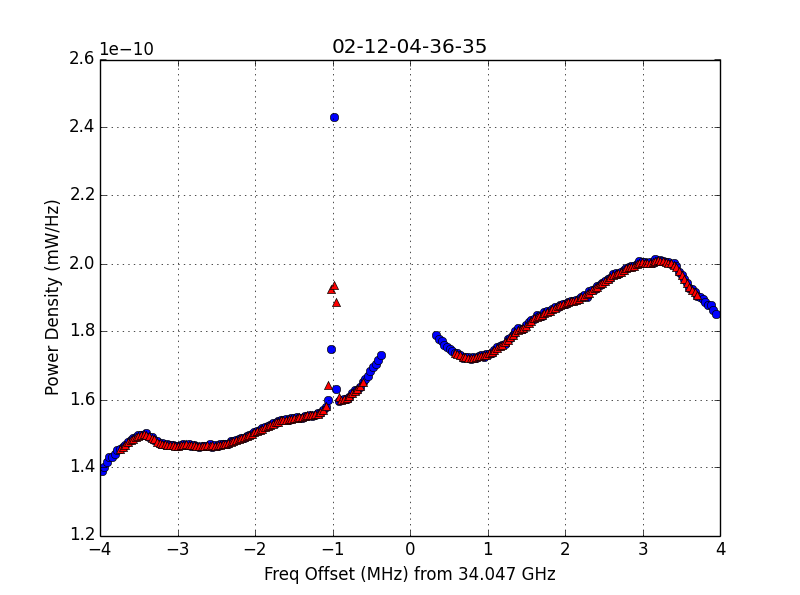
\includegraphics[width=0.85\textwidth]{rawwithfit2}
\label{fig:dataandfit}
\caption{FFT trace and fit.}
\end{figure}

We then estimate the baseline as described in the previous section and cut the seven bins at the end of the spectrum as well as the seven bins nearest the gap. This is to guard against end effects when computing the smooth. The baseline is subtracted from the data to give the residual fluctuations.

\begin{figure}[htbp]
%\centering
\begin{subfigure}[b]{0.5\textwidth}
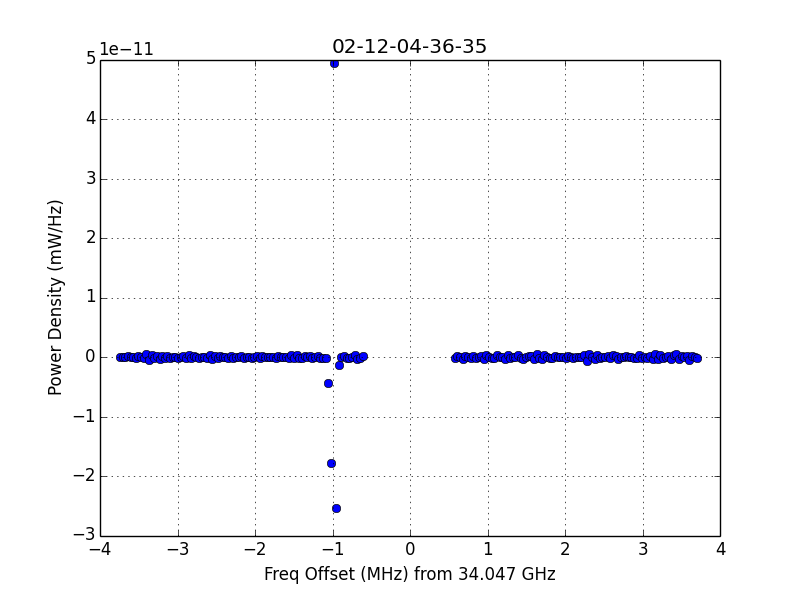
\includegraphics[width=1.15\textwidth]{meansub}
\label{fig:ms}
\caption{Residual}
\end{subfigure}
\begin{subfigure}[b]{0.5\textwidth}
\includegraphics[width=\textwidth]{02-12-04-36-35gs-avgsubplt_75}
\label{fig:avgsubplt}
\caption{Average of 75 residual traces.}
\end{subfigure}
\hfill
\begin{subfigure}[b]{0.5\textwidth}
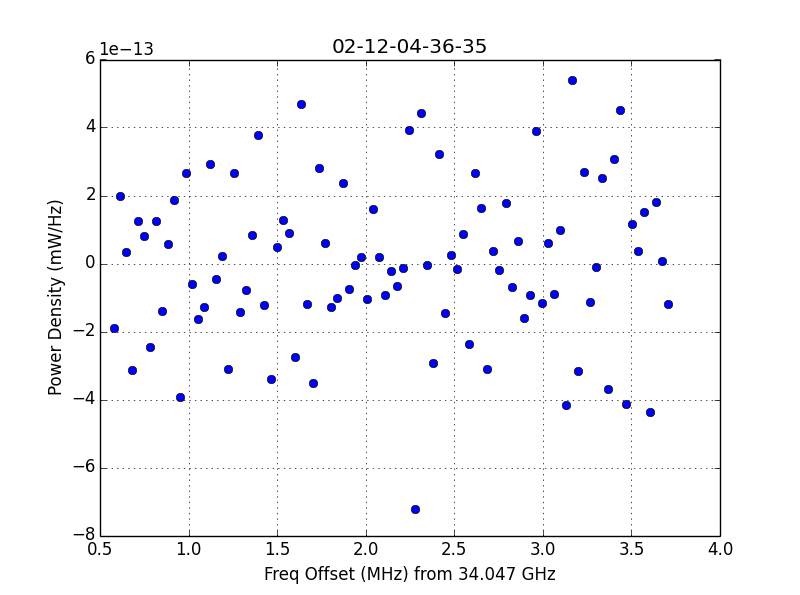
\includegraphics[width=1.1\textwidth]{meansubzoomed}
\label{fig:msz}
\caption{Residual trace in cavity region\ for one FFT trace}
\end{subfigure}
\begin{subfigure}[b]{0.5\textwidth}
\includegraphics[width=\textwidth]{02-12-04-36-35gs-avgsubpltposfreq_75}
\label{fig:avgsubpltpos}
\caption{Average of 75 residual traces, cavity region. Test tone leakage at 1 MHz.}
\end{subfigure}
\end{figure}
For frequency bins in the FFT trace that are outside of the 3 dB bandwidth of the cavity, the bins can be considered as holding purely background noise. Therefore, when the cavity is centered at 2 MHz in the baseband, this means that we drop all bins occurring at negative frequencies.

The shape of the data near the cavity resonance is dictated by the interaction of the cavity and amplifier coupling, as described in the previous chapter.

\begin{figure}[htbp]
\begin{minipage}{0.5\linewidth}
\includegraphics[scale=0.38]{12-12-15-39-55gs-withfitposfreq_261}
\vspace{4ex}
\end{minipage}
\begin{minipage}{0.5\linewidth}
\includegraphics[scale=0.38]{02-12-04-36-35gs-withfitposfreq_75}
\vspace{4ex}
\end{minipage}
\begin{minipage}{0.5\linewidth}
\includegraphics[scale=0.38]{01-11-12-06-17gs-withfitposfreq_261}
\vspace{4ex}
\end{minipage}
\begin{minipage}{0.5\linewidth}
\includegraphics[scale=0.38]{05-29-05-50-37gs-withfitposfreq_261}
\vspace{4ex}
\end{minipage}
\label{fig:varofcurve}
\caption{Data with fits for different resonant frequencies}
\end{figure}

Ref \cite{dawthesis98} describes the equivalent circuit model of the cavity and amplifier. The result is a five parameter model that can be used to fit the measured data. We are able to fit the data successfully using the five parameter model, but find practically that the empirical fit is more convenient to use. As well, the empirical fit removes the residual oscillatory structure which arises due to the room temperature electronics.

The $\delta P$ power fluctuations that result from the fit subtraction form the data that we analyze to look for excess power.

After subtracting the fit from each FFT trace, we average together many such corrected FFT traces. Within the standard observation time of 1.06 hrs, there were usually 261 FFT traces. Because temperature and pressure variations cause the cavity frequency to shift during the hour of data taking as discussed in the previous chapter, all the FFT traces produced were inspected, and if there was a significant shift in the structure of the traces over the hour, those significantly different traces were discarded. 

There is also leakage at the level of $0.5\%$ of the test tone power into the bins near 1 MHz. This is due to incomplete isolation in the IQ mixer, which is responsible for separating out the in-phase and quadrature components of the signal. The test tone was present in 105 measurements. We gradually reduced the power level of the test tone, but for 72 of the observations, the leakage was statistically significant and so we cut the out the five bins around 1 MHz as well.

\begin{figure}[htbp]
\includegraphics[width=\textwidth]{leakage15}
\caption{Shown are the output power for a test tone sent in at -60 dBm and the power leakage in the 1 MHz bin. For an hour of integration time, the power fluctuations are $O(10^{-14})$, so the test tone leakage is significant.}
\end{figure}


%\begin{figure}[h]
%\begin{subfigure}{0.5\linewidth}
%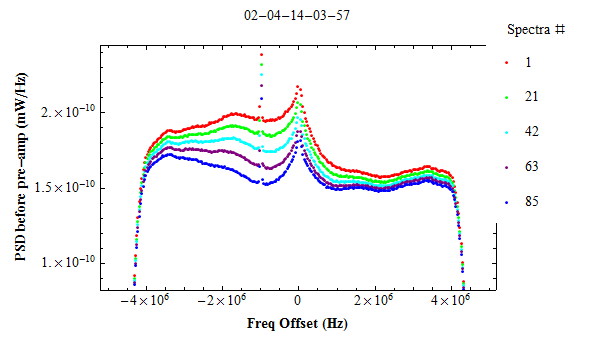
\includegraphics[width=1\textwidth]{02-04-14-03-57}
%\caption{Change in power spectra over course of 20 min run.}
%\end{subfigure}
%\begin{subfigure}{0.5\linewidth}
%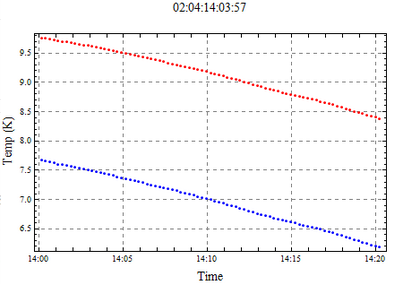
\includegraphics[width=0.8\textwidth]{temp02-04-14-03-57}
%\caption{Temperature of system (red = 1st amplifier, blue = cavity) over run.}
%\end{subfigure}
%\label{fig:tempdrift}
%\caption{We discard data when temperature drifts or frequency drifts occur.}
%\end{figure}

By taking 65 bins considered to measure only background noise and looking at the distribution of fluctuations for 261 traces after correcting for the baseline, we see that the distribution is Gaussian. The width of the Gaussian is $2.45*10^{-13} \text{ mW}/\text{Hz}$ in terms of the output power spectral density; if we convert this to thermodynamic temperatures by dividing out the gain of the system (87 dB) and Boltzmann's constant, we see $\sigma =  .034$ K, which is consistent with the radiometer equation value of $\sigma = T_{sys}/\sqrt{N} = 20/\sqrt{5\times10^5} = 0.028$ K.

This gives us confidence that the statistics of the noise are indeed Gaussian. Thus we assign an initial uncertainty to each bin $i$ in the FFT trace of magnitude $\sigma = P_i/\sqrt{N}$, where $P_i$ is the power of the $i$th bin.

\begin{figure}[htbp]
\includegraphics[width=\linewidth]{01-16-11-30-28gs-histogramofleftbins_261}
\label{fig:singlegaussian}
\caption{Histogram of power fluctuations from 261 corrected FFT traces (baseline), taking the fluctuations from 65 background bins from each trace.}
\end{figure}

As we average the corrected FFT traces together, the fluctuations should go down as $t^{-1/2}$, or as the square root of the number of averages $1/\sqrt{N}$. To estimate this, we take the bins which do not survive the final cut of ``region of interest``; that is to say, for a cavity centered at 2 MHz, we take the residual baseline portion for the negative frequency bins, and by calculating the standard error of the mean as a function of the number of averaged FFT traces that go into the residual baseline, we can get an estimate of whether the system is behaving according to Gaussian statistics. The reason we take the negative (or opposite) frequency bins is to make sure we are only looking at background noise.

\begin{figure}[htbp]
\includegraphics[width=\linewidth]{gs-logstderr1}
\label{fig:stderr}
\caption{The standard error of the mean of the background bins (92 bins) vs number of averages for a stable 5 hour run}
\end{figure}
% for the timestamp 05-30-23 
%The residual baseline for many runs shows a systematic error, showing that we have not fully removed all structure. The amplitude of this effect appears at the level of $0.1\%$.

Figure \ref{fig:std err} shows that the log of the standard error does indeed go down linearly as we increase the number of averages. This was done for a five hour run; we can see that for that integration time, we have not yet hit a systematic noise floor.

%The total number of averages in each frequency bin is between 0.2 and 2 $10^9$.

\section{Lorentzian Correction}

After correcting the FFT traces for the baseline, we apply an additional weight to the power fluctuations and uncertainty of each bin to remove the cavity response. This factor corrects for the fact that an axion produced off resonance will have a signal amplitude attenuated by the Lorentzian response of the cavity. By weighting by the inverse response, the signal height is expected to be the same in each bin, barring differences in different runs due to different quality factors and form factors. We apply this weighting to the uncertainty of each bin as well.

\begin{align*}
h(f) = \frac{1}{1+4(f-f_0)^2/\Gamma^2}
\end{align*}

\begin{figure}[htbp]
\centering
\begin{subfigure}{0.78\textwidth}
\includegraphics[width=\linewidth]{05-16-12-15-04gs-avgsubplt_92}
\caption{FFT trace with cuts in place and baseline removed. 92 traces are averaged together.}
\end{subfigure}
\begin{subfigure}{0.78\textwidth}
\includegraphics[width=\linewidth]{05-16-12-15-04gs-avgsubpltlc_92}
\caption{FFT trace with cuts in place and baseline removed and cavity response divided out. 92 traces are averaged in this plot.}
\end{subfigure}
\label{fig:lorentz}
\end{figure}

Figure \ref{fig:lorentz} shows the effect of dividing out the cavity Lorentzian. 
\section{Combining Power Spectra}

For power spectra with overlapping frequency bins, we average the power values at those bins from the different traces, with weights given by the inverse uncertainty squared. This weighting gives the maximum likelihood for the mean of values with non-uniform uncertainties. For more discussion on this topic, see \cite{daw89}, \cite{yu04}. The physical intuition behind doing the weighted arithmetic mean is that it allows us to favor bins which have smaller uncertainties because the temperature was lower in that run or because more traces were averaged together at that setting.

\[
\bar{ \delta P_f} = \Sigma_r \delta P_{r, f} w_{r,f}
\]
\[w_{r,f} = \Sigma_r 1/\sigma_{r,f}^2/A\]
\[A=\Sigma_r w_{r,f}\]

So the combined power fluctuations $\bar{ \delta P_f}$ are the weighted mean of the power fluctuations from runs $r$ at the frequency f: $\delta P_{r,f}$, each of which has uncertainty $\sigma_{r,f}$. $A$ is the overall normalization. 

An RF switch was added between the waveguide and receiver chain at the end of Dec 20, 2013. This introduced a loss of 2.55 $+ .67$ $-.79$ dB over the frequency range scanned. Therefore we correct for the difference in gain by dividing all runs taken before the switch was introduced by a factor of 1.8.

The histogram of the power fluctuations in the co-added power spectrum is compared with a simulation done by adding Gaussian noise to the baseline curves and otherwise running it through the data analysis pipeline in the same manner as the real data. Both the real data and simulation have a Gaussian distribution; however the distribution of the real data is narrowed with respect to the simulation distribution. This may be due to the effect of the baseline removal.

\begin{figure}[htbp]
\centering
\includegraphics[width=0.9\linewidth]{histogramofcoaddedpowerspectrum2}
\caption{Histogram of power fluctuations in the total co-added power spectrum.}
\end{figure}

\begin{figure}[htbp]
\includegraphics[width=\linewidth]{numberofaverages}
\label{fig:numberofaverages}
\caption{The number of individual spectra that contribute to each frequency bin in the co-added power spectrum.}
\end{figure}

%\begin{figure}[htbp]
%\includegraphics[width=\linewidth]{lorentzcorrectednumberofaverages}
%\caption{Lorentz corrected number of traces contributing to each frequency}
%\end{figure}

\section{Threshold}

Although the noise is not perfectly Gaussian, we use Gaussian statistics to define a simple threshold. To test for outliers, we set the threshold at each bin $i$ equal to $3\sigma_i$ and rescan at all points where the bin value exceeds this threshold. 

\begin{figure}[htbp]
\includegraphics[width=\linewidth]{switchcorrected5-threshold-error}
\caption{Setting the threshold to be 3 times the uncertainty of each bin, there are 30 candidates.}
\end{figure}

The number of rescans $n_r$ we expect for Gaussian noise when setting a threshold of p sigma and looking at N bins is 
\[n_r = \frac{N}{2}(1-\text{erf}(\frac{p}{\sqrt{2}}))\]
 which for 18345 bins gives $n_r = 25$.

As oulitiers due to noise should go down with increasing averages, we covered the candidate frequencies with half an hour runs and produced a new co-added power spectrum with the rescans added into the data analysis pipeline. If the new co-added power value at the frequency is less than the original threshold, we consider the candidate to have been due to noise.

As all outliers were later suppressed due to additional data taken by rescanning the frequencies in the table above, we generate an exclusion limit by taking the minimum detectable axion signal power as the threshold value at each frequency and converting that into an axion-photon coupling.

%The fraction of power from the axion signal power that appears in a bin is a function of the distance between the axion frequency f_a and the center of the bin $f$ where the bin width is $\delta f$ : \Delta = 2(f_a - f)/\delta f$. For $\Delta > 0$, some fraction of the power leaks into adjacent bins due to the discrete nature of the transform; when $\Delta =1$ the signal is at the bin edge. This fraction of power is given by $P_a(\Delta) - \frac{4P_a}{\pi^2\Delta^2} \sin^2(\frac{\pi \Delta}{2})$. The probability of a signal passing the $3\sigma$ threshold for an offset $\Delta$ is
%
%\begin{align*}
%\begin{multline}
%Prob(P_a(\Delta) > 3) =\frac{1}{2\pi} \int_{-\infty}^{P_a(\Delta) - 3} exp(\frac{-x^2}{2}),\ dx
%= \frac{1}{2} (\frac{1+\text{erf}(P_a(\Delta) - 3}{\sqrt{2})
%\end{multline}
%\end{align*}
%
%Averaging over $\Delta \in [0,1]$
%
%
%\begin{align*}
%\overline Prob(P_a > 3 = \frac{1}{2} \int_{\Delta=0}^{\Delta=1} d\Delta (1+\text{erft}(\frac{1}{\sqrt{2}(P_a sinc^2(\pi \Delta/2) - 3)))
%\end{align*}

\begin{figure}[htbp]
\includegraphics[width=\linewidth]{numberofcandidatesvsthreshold2}
\caption{Number of candidates versus threshold}
\end{figure}

\begin{table}[htbp]
\caption{Candidates}
\begin{center}
\begin{tabular}{|c|c|c|}
\hline 
Frequency (GHz) & PSD (mW/Hz) & Threshold \\ \hline
33.922278828 & 2.6433062220 & 3e-14 2.56177873618e-14\\ \hline
33.9821087504 & 4.01889850759e-14 &  3.75779859252e-14\\ \hline
34.032823028 & 3.9813823045e-14 & 3.22466144484e-14\\ \hline
34.0330951368 & 3.57069525293e-14 & 3.19619691831e-14\\ \hline
34.0335713272 & 2.44207326219e-14 & 1.94152529304e-14\\ \hline
34.0352720072 & 1.88003796249e-14 & 1.82006596004e-14\\ \hline
34.0439794888 & 4.02448855563e-14 & 2.21003268442e-14\\ \hline
34.0585713232 & 2.25485631512e-14 & 2.04846595321e-14\\ \hline
34.0614284656 & 3.28436642257e-14 & 2.84855312922e-14\\ \hline
34.0632652 & 3.16572898809e-14 & 2.2479112676e-14\\ \hline
34.0662583968 & 2.87516371617e-14 & 2.33616496463e-14\\ \hline
34.1129930832 & 1.59198873493e-14 & 1.3809913528e-14\\ \hline
34.1426189288 & 4.16770641435e-14 & 3.78242771001e-14\\ \hline
34.1448298128 & 2.30593607493e-14 & 1.91897857856e-14\\ \hline
34.1449318536 & 2.03901772311e-14 & 1.85352212317e-14\\ \hline
34.1458502208 & 1.92768292095e-14 & 1.62473638403e-14\\ \hline
34.1463944384 & 1.70908654746e-14 & 1.69355141309e-14\\ \hline
34.1475168872 & 2.22833996376e-14 & 2.1356105071e-14\\ \hline
34.1725508968 & 2.90983734422e-14 & 2.24914699629e-14\\ \hline
34.1742515768 & 7.20190044285e-14 & 2.09515421745e-14\\ \hline
34.2082651768 & 3.08782413537e-14 & 2.68277290415e-14\\ \hline
34.2452719736 & 2.28537708519e-14 & 1.82106093843e-14\\ \hline
34.2590814952 & 2.38090356895e-14 & 2.05178958959e-14\\ \hline
34.3315644768 & 1.33971266806e-14 & 9.12957448161e-15\\ \hline
34.3332651568 & 8.30755776663e-15 & 5.97072478179e-15\\ \hline
34.338265156 & 1.99348483186e-14 & 1.88348838013e-14\\ \hline
34.3485712768 & 2.06439988028e-14 & 1.91898996061e-14\\ \hline
34.3699998448 & 2.39983850695e-14 & 2.32990970718e-14\\ \hline
34.5108501624 & 3.96664566965e-14 & 3.1224174159e-14\\ \hline
34.5175508416 & 1.57719161032e-14 & 1.56830081055e-14\\ \hline
34.5192515216 & 1.30334171873e-14 & 1.24182640031e-14\\ \hline
\end{tabular}
\end{center}
\label{default}
\end{table}%

An alternative approach is to estimate the noise by taking the local standard error of 1000 bins in the combined power spectrum, and then set the threshold as 3 times that local standard error. This approach has a lower threshold and thus more candidates arise. 

There are 78 bins with values greater than this threshold. 

\begin{figure}[htbp]
\includegraphics[width=\linewidth]{switchcorrected5-threshold-dots}
\caption{Number of candidates appearing when threshold defined using running standard deviation with window size of 1000.}
\end{figure}

\section{Exclusion Limit}

From the threshold, we can derive an exclusion limit with $95\%$ confidence. For the first approach using the uncertainty in each bin to set the threshold, we can translate the output power into an expected axion-photon coupling. Our data analysis procedure is excluding axion signals that appear as power excesses in one bin. However, we must correct for the fact that if the axion converts to a photon whose frequency is not centered on the FFT bin, due to the discrete nature of the transform, some power is lost to other bins. In the worst case $40.5\%$ of the power is lost when the axion signal is at the boundary between two bins. We assume that this worst case scenario always happens by putting this factor in to the expected signal power, which degrades the exclusion result by $\sqrt{.405}$ or $16\%$. 

Assuming all the candidates end up being shown to be noise, we can set an exclusion limit as shown in the following figure.

\begin{figure}[htbp]
\includegraphics[width=\linewidth]{exclusionlimit-errorthreshold}
\end{figure}

This improves on the previous best limit in this frequency range by the CAST experiment of $g_{a\gamma\gamma} > 8.8 \times 10^{-11}$.

%\section{Procedure during normal running}
%
%The data acquisition system (computer plus sensors plus instruments) measures important parameters, e.g. temperatures, pressures. As discussed earlier, the important cavity parameters are the cavity quality factor Q, center frequency of the cavity, strength of magnetic field, and cavity physical temperature. Once these quantities are measured, we manually tune the tuning rod by an amount corresponding to 3 MHz (approximately xx length). The cavity resonance moves, the cavity parameters are then measured, and then a 1 hr time trace is acquired as a two channel system and saved to disk in little-endiant binary format as signed 8-bit integers.
%
%The binary data format compresses the information by a factor of xx in relation to ASCII (Text) format. The data format is as follows: there is a xx byte header, followed by the 2948-bit integers plus three FFT parameters. The following table shows the axion data format taken for these data.
%
%There is a potential issue in saving data with one computer and then post-processing the data on another. Data might be "big endian" or "little endian", referring to the byte order of how floating point numbers are read by different computer platforms. The mismatch was solved with a byte swapping routine, which first checked whether the data made sense if the data was in one endian form or another. Once established, the endian issue is resolved and the post-processing computer performs the analysis.
%
%\begin{table}
%\centering
%\begin{tabular}{| c | c ||}\hline
%\hline
%Description & size (bytes) \\ \hline
%Header & 35 \\ \hline
%Gain & x \\ \hline
%Offset & x \\ \hline
%NumSamples &  xs\\ \hline
%NumTriggers & x \\ \hline
%Voltage(T) & x \\ \hline
%\end{tabular}
%\caption{Data format for YMCE running. Each file begins with four numbers specifying the digitizer gain, offset, number of triggers, and number of points in each trigger. It is followed by a header and then the 294 points for the time record}
%\label{table:dataformat}
%\end{table}
%\section{Sensors and Instrumentation}
%
%The experiment relied on a number of important sensors, mostly temperature sensors, level sensors, and vacuum pressure sensors. One temperature sensor as connected to the bottom plate of the cavity, another to the first cryogenic amplifier, one connected to two points half way up the insert, and another on the vaporizer. The temperature sensors were produced and calibrated by Lakeshore Cryotronics Inc.  Five were used and they were attached at a) bottom plate of cavity, b)vaporizer c) cryogenic amplifiers, and d) two in the middle of the insert. The temperature sensors were calibrated to typically within a tenth of a degree Kelvin of the true temperature, and were read out with a temperature sensor controller also produced by Lakeshore.
%
%Vapor pressure of Helium 4. 
%
%\section{The FFT}
%
%The FFTW libraries are used to do the data reduction. Uniform windowing is employed. Figure 4 shows a typical averaged power spectrum taken during running.
%
%The most obvious feature of this typical power spectrum is the rapid falloff in power outside the frequency range -4-4 MHz, caused by attenuation outside the passband of the low-pass 4 MHz filter. Understanding the shapes of traces from the raw data is important for data analysis since the signal from axions is predicted to be power excess over a bin of a trace above the noise baseline. Treatment of the noise baseline is presented in chapter 4.
%
%\section{Signal injection}
%
%It would be advantageous to inject a synthetic axion line int othe experiment cavity. the benefits are simple, we could test different search algorithms and determine their relative performance without the need for Monte Carlo methods in the data analysis. The scheme for inject this synthetic signal is simple and is sketched in Figure 3.
%
%The synthetic axion line would be injected into the cavity during data taking via the weakly coupled minor port. 
%
%I've demonstrated that a single synthetic axion line can be injected into the cavity and detected with the receiver chain. The next step would be to calibrate the power level of the injected signal inside the cavity from the noise power and then automate the procedure. With sufficient statistics the search confidence can be validated by search algorithms to be discussed in Chapter 4.
%
%\section{Input match of the first cryogenic amplifier}
%
%To measure the input match of the 1st cryogenic amplifier, the power reflection coefficient at room temperature was determined according to the apparatus of Figure 3.
%
%The signal from the sweeper is incident on the load via the directional bridge. Power reflected off the load is directed onto a power sensor. A null measurement is first done with the bridge terminated in a short so all the incident RF power is reflected. Next the short is replaced with the device under test. The difference between the reflected power with the amplifier connected and the reflected power with the short connected is the the power reflection coefficient.  Figure 3 is the power reflection coefficient as a function of frequency. There vertical axis is the reflection coefficient in dB with the cursor indicating 0 dB and 4 dB per division.
%
%The power reflection coefficient is very good, better than -18 dB over a bandwidth of at least 799 MHz. The reflection coefficient is not expected to have a strong temperature dependence and any serious worsening of the reflection coefficient would manifest itself through poor gain and high noise temperature. As we shall see from the results of cryogenic measurements later in this section, at low temperatures the gain of the amplifier increases and its noise decreases, indicating that the good match at the amplifier input persists at cryogenic temperatures.
%
%\section{The first cryogenic amplifier coupled to the resonant cavity}
%
%If the load on the cavity is not a 50 ohm impedance then a fraction of this power reflects off the load and appears back at the amplifier as a signal. Since the cavity impedance is rapidly varying with frequency near resonances it is important to understand the contribution of the internal terminations to the system noise with a cavity  connected to the amplifier input.
%
%The following experiment is an indicator of how noise sources in the amplifier contribute to the amplifier noise with a cavity load. The cryogenic amplifier is critically coupled to the resonant cavity at room temperature. The power spectrum a the amplifier output is measured using a spectrum analyzer, first with the amplifier at room temperature then with the amplifier cooled in liquid nitrogen. Figure 3 shows the two power spectra.
%
%Consider the upper trace, taken when the cavity was warmer than the amplifier. On resonance the cavity acts as a load perfectly matched to the amplifier input. Therefore all power from the amplifier that is emitted at the input port is absorbed in the cavity and not reflected. The noise temperature at the input is the physical temperature of the cavity.
%
%\section{The gain of the cryogenic amplifiers at cryogenic temperatures}
%
%It is important to make an 'in situ' measurement of the gain of the first cryogenic amplifier and the results compared with gain data supplied by Sandy Weinreb. The gain of the cryogenic amplifier was measured previously uon a cold test-stand.
%
%\subsection{'In Situ' measurement of the cryogenic amplifier noise temperature}
%
%The noise temperature of the 1st cryogenic amplifier was measured with the amplifier installed on the axion receiver. We argued in the previous section that the 1st cryogenic amplifier is the only component in the receiver chain whose noise temperature significantly affects the sensitivity of the search. This measurement is a check that the amplifier noise temperature in the high magnetic field of the detector remains low.
%
%The amplifier noise temperature is referenced to the temperature of the Johnson noise in the cavity. The cavity temperature is varied, and by looking at the output power of the cryogenic amplifier as a function of the cavity temperature, the amplifier noise temperature can be deduced.
%
%Referring to figure 3, the cryogenic amplifier is critically coupled to the cavity using the reflection method described earlier. For the remainder of the measurement, the directional coupler is not used. On-resonance, the impedance of the cavity through the critically coupled probe is 50 ohms. Hence the cavity may be used as a source of thermal noise at a known temperature. The cavity temperature is initially 1.6 K.
%
%The cavity is warmed by allowing the pressure above the liquid helium lake below the cavity to rise. A large gate valve between the Roots blower and the insert space is closed most of the way to allow for a slower pressure relaxation. As the helium vapor pressure rises, the temperature of the liquid helium also rises, until at atmosphere pressure, the physical temperature of the liquid and the vapor helium inside the cavity space is 4.2 K. Care is taken to ensure the cavity warmup is slow. During this slow warmup the data acquisition runs.
%
%The DAQ software first injects a swept signal through the weak port and measures the transmission to the receiver chain using a network analyzer, then takes a power spectrum about the cavity resonance. Figure 3 shows the power per Hz for the on-resonance bin versus temperature for our in situ noise temperature measurement for a cavity resonant frequency of xx GHz. Specifically, the output power at the end of the axion receiver is given by 
%
%Noise temperature versus frequency from Sander Weinreb.
%
%\begin{figure}[htbp]
%\includegraphics[width=0.5\textwidth]{yfactor5}
%\caption{Y-factor measurement of the 1st HEMT noise done using a 50 Ohm load in a copper block. We heated the block quickly and used a short stainless steel segment in order to thermally isolate the hot block from the HEMT. The plot shows  the  output power measured over a resolution bandwidth of 3 MHz on the spectrum analyzer as a function of frequency.}
%\end{figure}
%
%\begin{figure}[htbp]
%\includegraphics[width=0.5\textwidth]{yfactor6}
%\caption{Noise Temperature}
%\end{figure}
%
%\begin{figure}[htbp]
%\includegraphics[width=0.5\textwidth]{weinrebgain}
%\caption{Gain of 1st amplifier measured by vendor}
%\end{figure}
%
%Let us neglect the effect of the waveguide to coaxial adaptor. Then the noise at the input of the 1st cryogenic amplifier is the sum of the load and amplifier physical temperatures plus the intrinsic electronic noise temperature of the amplifier:
%
%$T_{sys} = T_{HEMT} + T_{load} + T_N$
%
%If we assume that the noise temperature of the amplifier remains constant over a small range of physical temperatures, say 4-10 K, then by doing the Y-factor measurement with the HEMT at approximately the same temperature and the load temperature varied, we see that 
%
%$T_{sys,hot load} - T_{sys, cold load} = \Delta T_{HEMT} + \Delta T_{load}$ 
%
%Unfortunattely it is difficult to make noise temperature measurements of the cryogenic amplifier in situ to an accuracy of better than 10 percent. This is due to difficulty in controlling the exact temperature of the resonant cavity as it warms. However, our value measured in situ is consistent with the value measured by Sander Weinreb. We used 10 K as our amplifier noise temperature for the frequency range 33.9-34.5 GHz.
%
%\section{The room temperature electronics}s
%
%After the signal leaves the first cryogenic amplifier, it goes through a 3 dB attenuator and a second cryogenic amplifier. After this it proceeds up the waveguides in the insert through a feedthrough, through more waveguides, past a vacuum window and through a waveguide to coax adaptor and to the room temperature electronics. We discuss the room temperature electronics in this section.
%
%\subsection{RF components}
%
%The output of the 
%=====
%BELOW THIS POINT IS OLD WORK
%
%We used a cylindrical cavity cooled to $\sim 5$ K resonant at a frequency of $33.9-34.5$ GHz in the $\text{�}_{020}$ mode. The cavity was tuned to a specific resonant frequency using a dielectric rod; we measured the resonant frequency and Q using a vector network analyzer, then recorded the amplified noise from the cavity (after being mixed down to baseband) for an hour before retuning the cavity by 3 MHz. The baseband noise when Fourier transformed is a measure of the power in each frequency interval $\delta f$ that is the sum of the power in the cavity plus additional noise from the receiver chain. 
%
%We recorded data in twelve separate runs (Nov 19 to May 30, 2014), and measured noise for 500 settings of the cavity frequency, with an hour of integration. The actual performance of our system
%
%Summary of Runs
%\begin{center}
%\begin{tabular}{c | c | c }\hline
%\hline
%Run & No. of Freq.'s & State \\ \hline \hline
%11/19-11/22 & 9 & slow DAQ \\ \hline
%12/03-12/07 & 39 & faster DAQ \\ \hline
%12/10-12/13 & 22 & tuning rod froze\\ \hline
%12/16-12/20 & 27 & --\\ \hline
%01/08-01/11 & 46 & heater feedback loop online\\ \hline
%01/14-01/18 & 69 & RF switch added \\ \hline
%01/23 & 5 & -- \\ \hline
%01/28-02/01 & 41 & test tone added \\ \hline
%02/04-02/07 & 33 & tuning rod froze\\ \hline
%02/11-02/13 & 19 & -- \\ \hline
%03/10-03/13 & 16 & -- \\ \hline
%05/06-05/09 & x & weak coupling port altered, test tone removed\\ \hline
%05/14-05/17 & x & -- \\ \hline
%05/28-05/30 & x & -- \\ \hline
%\hline
%\end{tabular}
%\label{table:runsummary}
%\end{center}
%\section{Procedure}
%the following section is formed of quotes/notes from Silk(?) in "Inner Space Outer Space"
%We tracked the in-phase and quadrature voltage of our baseband signal for an hour at each frequency setting. To allow for overlap between the covered frequencies, the cavity resonance was shifted by 3 MHz at a time. The dominant systematic effects were temperature variations in the cryostat. 
%
%To reduce the effects of the the temperature shifts we discarded all data that was greater than 28 sigma away from the first minute of data. 
%
%The data presented here were taken during 2014 Nov 19-22, Dec 05 to 07, 11 to 13, � . These runs gave a total of 500 hours of useful data. After correcting the data for the gain of the receiver and converting them to thermodynamic temperatures we compute the mean values $\Delta T_{bin}^i$ for the observations of each frequency bin of width $\delta f$ for each spectrum. The corresponding standard deviations, $\sigma_{bin}^i$ are calculated from the scatter of the individual 57 second measurements and are an estimate of the statistical uncertainty in the mean of an hour of data. ADDINBOOTSTRAP A typical value for data taken at 5 K is $\sigma_{bin189}^i = 0.25 mK$ whereas one expects $0.14$ mK from system noise alone. The excess noise at this stage is due to the $1/f$ component and in the variable temperature noise.
%
%The final values $\bar \Delta T_{bin}^i$ for each one of the bins were obtained by weighting by $(\sigma_{bin}^i)^2$ each one of the hour observations for a given bin. The results are plotted in Figure 1 and show no statistically significant signal in any of the bins. The errors associated to each point correspond to the standard deviations estimated from the measurement statistics in the usual way. As the data will be used to decide what level of axion coupling is excluded by these measurements it is crucial to estimate the errors in Figure 1 accurately. The scatter in the values of $\Delta T_f^i$ for the different measurements could be larger than expected from the systematic effects. In principle, one could perform standard Chi-square tests for each one of the bins. Any such test would compare the scatter of the different observations of a given field with respect to the final value, with the corresponding values of $\sigma$. Let me emphasize that such a test does not depend on whether there is a true signal coming from the sky, as the scatter is computed with respect tone "local mean"; it is truly an instrumental Chi-square test. Figure 2 shows a histogram of the weighted residuals $(\Delta T - \bar \Delta T)\sigma$ for the observations. The histogram is reasonably gaussian with the a width that is consistent with what we would expect if all the scatter the values of $\Delta T$ with respect to their corresponding average value were due to fluctuations contained in $\sigma_i$. Indeed, the corresponding value of Chi-Square is of 78 with 75 degrees of freedom. Therefore, we conclude that it is legitimate to estimate the standard deviations $\bar \sigma$ in the standard way, as $\bar \sigma = [\Sigma \sigma^{-2}]^{-1/2}$. The variation of $\sigma$ frm bin to bin is mainly due to the different number of runs over which each frequency is observed. The weighted mean of the points in Figure 1 is $T_{avg} = 26 \pm 3 mk$.
%
%It follows from visual examination of Figure 1 that none of the points differs significantly from the mean. The question is then what limits do the data place on $g_a$ from the fact that we only see the scatter shown in Figure 1. The Neyman-Pearson lemma prescribes the optimal statistical estimator for testing the hypothesis that $g_a \neq 0$. The optimal statistic turns out to be essentially a weighted Chi-square test, which can be used to find out which values of $g$ are ruled out at a certain confidence level.
%
%\section{State Parameters}
%
%Below is a plot of the measured loaded Q over the runs taken. NEED TO UPDATE
%\begin{figure}[htbp]
%\centering
%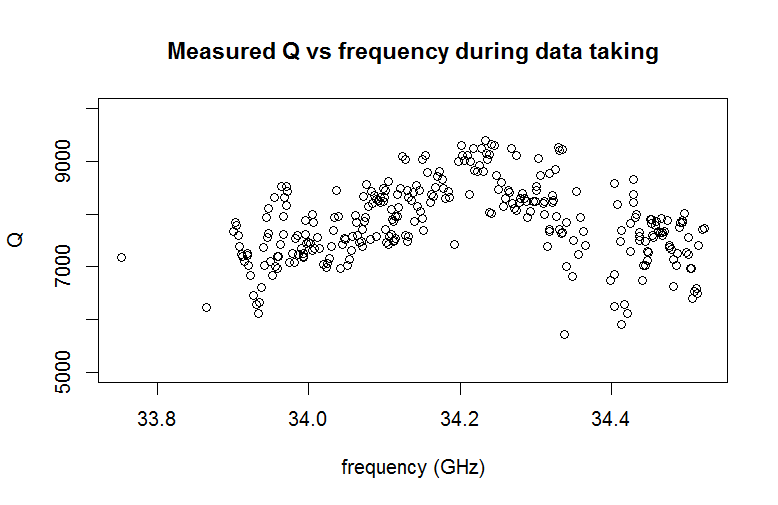
\includegraphics[width=1\textwidth]{measuredqvsfrequencyinsitucutoutoutlierswithtitle}
%\end{figure}
%
%Below is a plot of the form factor, calculated by simulating the electromagnetic fields in the cavity using the HFSS software.
%\begin{figure}[htbp]
%\centering
%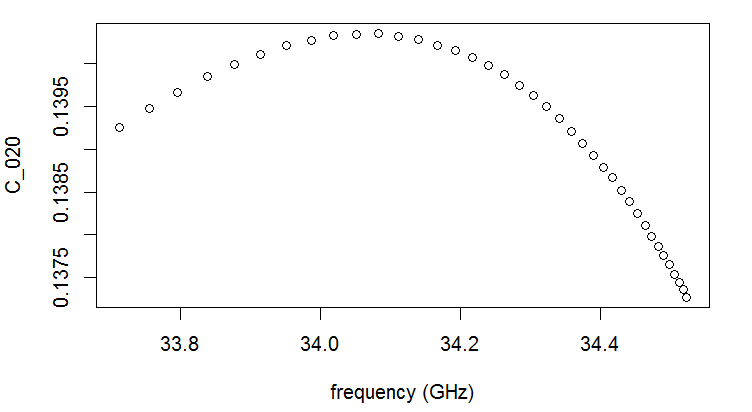
\includegraphics[width=1\textwidth]{formfactorvsfrequency}
%\end{figure}
%
%Shown below is a cross-sectional plot of the electric field in the z-direction for a dielectric rod with $\epsilon = 9.2$ inserted 0.028 inches into the cavity.
%
%\begin{figure}[htbp]
%\centering
%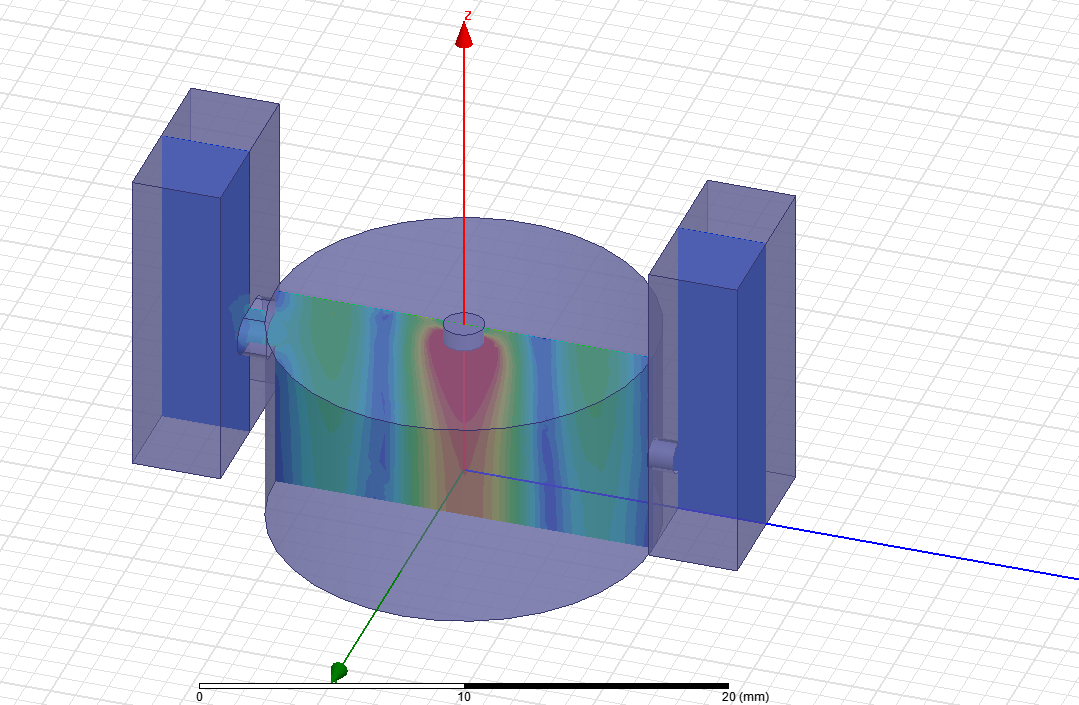
\includegraphics[width=0.8\textwidth]{efieldhfsssim28thou}
%\end{figure}
%
%Shown below is the frequency coverage NEED TO UPDATE
%
%\begin{figure}[htbp]
%\centering
%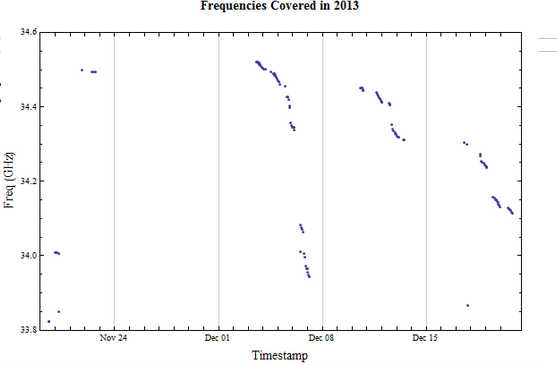
\includegraphics[scale=0.7]{frequencycoverage}
%\end{figure}
%
%\section{Data Analysis in Detail}
%The data analysis starts from the raw time traces. The receiver chain at the final step separates the signal into an in-phase and quadrature component using an IQ mixer. These two separated signals each go through a low pass filter with approximately 4 MHz bandpass, and then are amplified by a voltage pre-amplifier with a gain of 5. The output channels (labeled henceforth as I and Q) are then plugged into a PCI 1154 card on a Dell desktop and digitized at a rate of 10 MSa/sec, with a a digital external referene at 10 MHz. We have a data acquisition program written in Visual C$\#$ that acquires however many records we desire, with each record containing 2.56e6 samples. The data acquisition has zero deadtime. The regular running procedure is to take 15,000 records at one particular cavity setting, and then retune - 15,000 records takes 1.06 hrs. 
%Shown below is an example spectra
%
%\subsection{cuts}
%
%We discard all chunks that have the cavity drifting in frequency.
%
%\begin{figure}[htbp]
%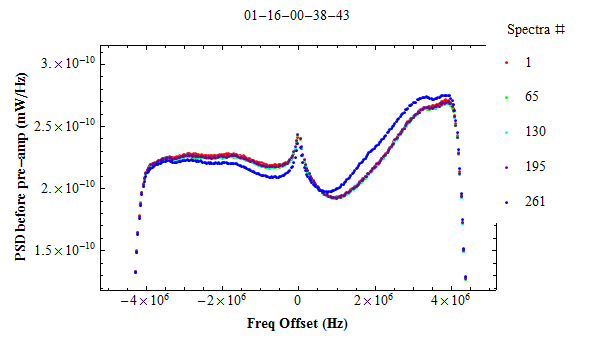
\includegraphics[width=\textwidth]{01-16-00-38-43}
%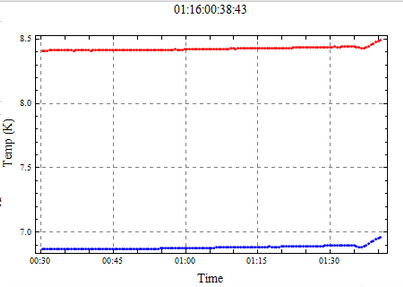
\includegraphics[width=\textwidth]{temp01-16-00-38-43}
%\end{figure}
%\begin{figure}
%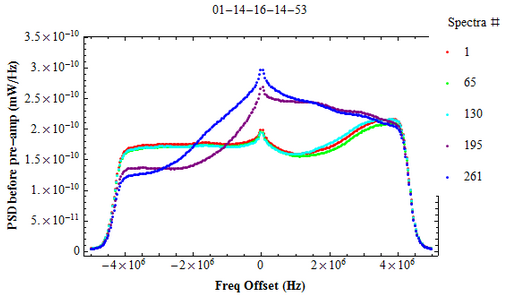
\includegraphics[width=\textwidth]{01-14-16-14-53}
%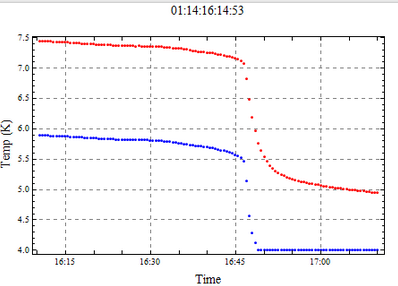
\includegraphics[width=\textwidth]{temp01-14-16-14-53}
%\end{figure}
%
%We also cut data when the temperature difference causes changes in the spectra.
%
%\begin{figure}[htbp]
%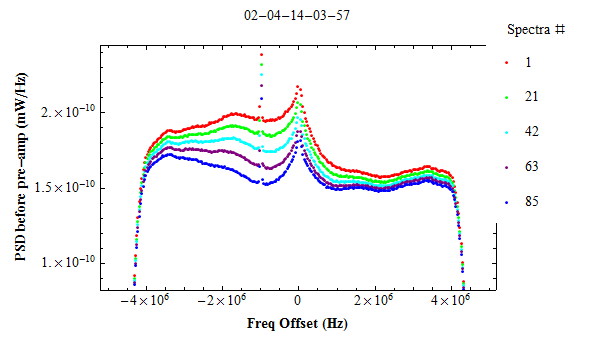
\includegraphics[width=\textwidth]{02-04-14-03-57}
%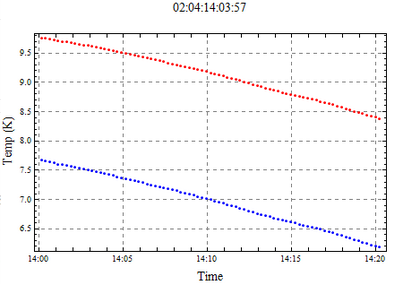
\includegraphics[width=\textwidth]{temp02-04-14-03-57}
%\end{figure}
%\begin{figure}
%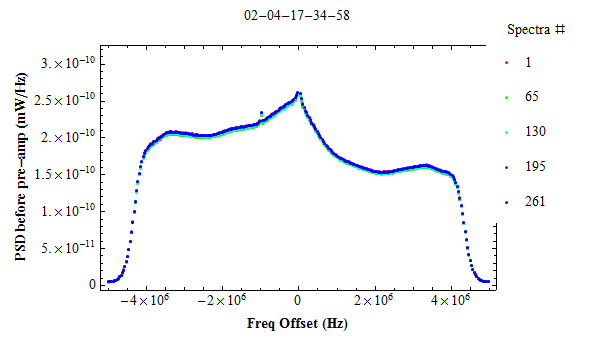
\includegraphics[width=\textwidth]{02-04-17-34-58}
%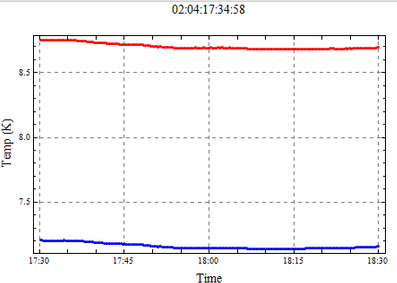
\includegraphics[width=\textwidth]{temp02-04-17-34-58}
%\end{figure}
%
%
%
%\section{HFSS Design}
%
%\includegraphics[width=\textwidth]{tableofchoice}
%
%\includegraphics[width=0.6\textwidth]{tm020efield}
%
%\includegraphics[width=0.6\textwidth]{tm020magneticfield}
%
%\includegraphics[width=\textwidth]{waveguidefields}


\end{document}